
\documentclass[11pt]{article}

\usepackage{amsmath}
\usepackage[utf8]{inputenc}
\usepackage{geometry}
\geometry{a4paper}
% \geometry{margin=2in} % for example, change the margins to 2 inches all round

\usepackage{graphicx} % support the \includegraphics

\title{TSRT14 --- Lab report}
\author{Group ID: xxx}
%\date{} % Activate to display a given date or no date (if empty),
         % otherwise the current date is printed 

\begin{document}
\maketitle
\newpage
\section{Data collection}
The data for this lab was gathered at a scheduled 30-minute session, where the task was to arrange seven microphones in two fundamentally different configurations chosen by the group, and record the sound emitted from a robot which followed a drawn out path in a stage, in order to localise it. The first configuration chosen was to evenly space the microphones around the stage as pictured in Figure 1. The second was to evenly space them on just one side of the stage as shown in Figure 2.
\begin{figure}[h!]
\centering
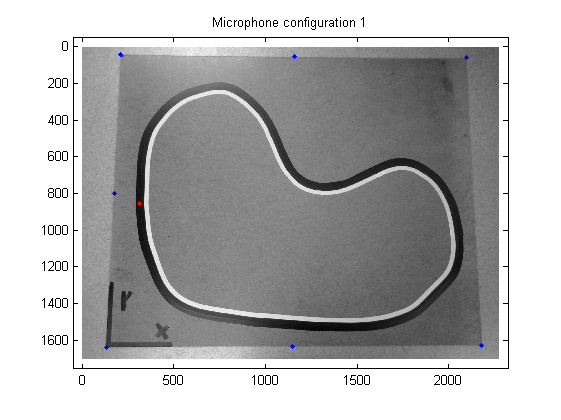
\includegraphics[width=\textwidth]{microphone_configuration_1.png}
\caption{First microphone configuration, believed to be the better one.}
\end{figure}
\begin{figure}[h!]
\centering
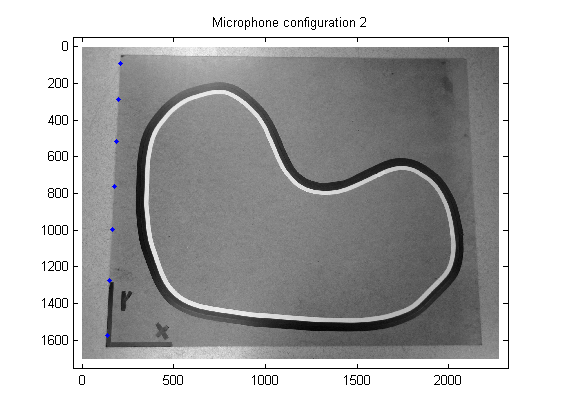
\includegraphics[width=\textwidth]{microphone_configuration_2.png}
\caption{Second microphone configuration, believed to be the worse one.}
\end{figure}
\newpage
The first was chosen as the configuration believed to be best, since it gathers data in the most even way, so that no "blind spots" would occur. Since this configuration is not always possible in real world examples, an easier configuration was chosen as the second one. These two represent very different approaches to the problem.\\\\
A calibration configuration was also set up, in accordance with the lab PM. Here the microphones were laid out in an arc with the same distance (0.7 meters) to the robot, while the robot emitted its sound at roughly 0.5 second intervals for 45 seconds.
\section{Localisation}
\subsection{Calibration}
The calibration data from the data collection session was used to estimate the spatial error for the localisation. It was calculated in the following way:

\begin{align*}
e_k = \text{tphat}_k-\text{mean}(\text{tphat}, 2)\\
k \in \{1,...,7\}
\end{align*}

This was then compared to a corresponding normal distribution, as shown for two microphones ($k=2$ and $k=6$) in Figure 3. 

\begin{figure}
\begin{center}
  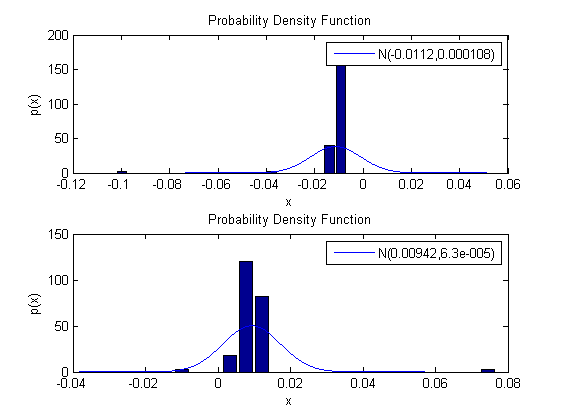
\includegraphics[width=\textwidth]{calibration_ndist_2_and_6.png}
  \caption{Spatial error for two of the microphones, 2 and 6 from the top.}
  \end{center}
\end{figure}


\subsection{Signal modeling}

%\subsection{Experiments}
%The obtained noise from the calibration was used as noise for the sensormod model. This yields a model that is close to the real life %results, since it contains noise with the same parameters as measured. 

\subsection{Configuration analysis}
In order to determine which of the microphone configurations is better, a configuration analysis is applied. This can be done in two different ways, the first one being Non-linear Least Squares (NLS), the second Cramér-Rao Lower Bound (CRLB). The CRLB approach is used here. The result of this on the first configuration (Figure 1) gives a plot with a clear minimum which indicates a good configuration, shown in Figure 4.\\
\begin{figure}
\begin{center}
  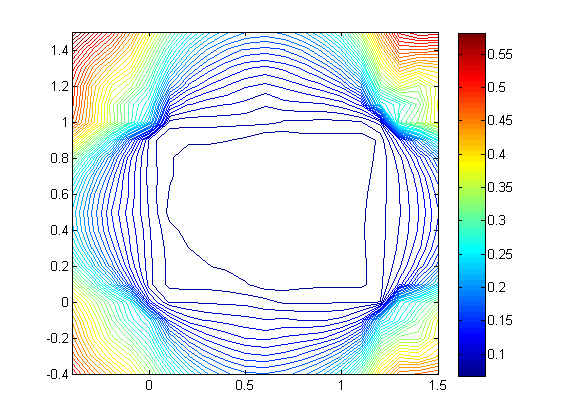
\includegraphics[width=\textwidth]{crlb_1.png}
  \caption{Cramér-Rao Lower Bound configuration 1.}
  \end{center}
\end{figure}
The result of this on the second configuration (Figure 2) gives a plot (Figure 5) with no distinct minimum which indicates a bad configuration. This configuration could be a bit better in hindsight, since it's virtually useless as it stands right now. It could be improved  for example by positioning the microphones around a corner.
\begin{figure}
\begin{center}
  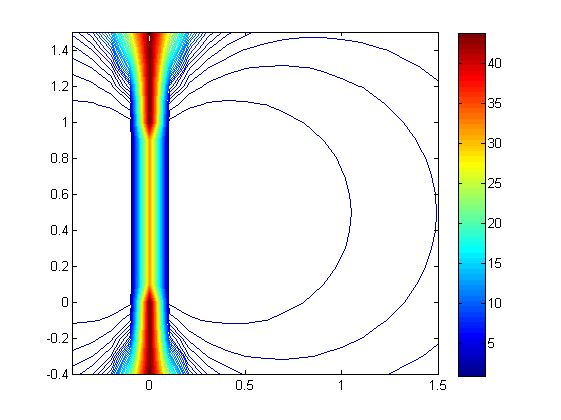
\includegraphics[width=\textwidth]{crlb_2.png}
  \caption{Cramér-Rao Lower Bound configuration 2.}
  \end{center}
\end{figure}


\subsection{Localisation}
The localisation of the robot was done in two different ways, one using a TDOA approach, and one using NLS using Gauss-Newton.

\subsubsection{TDOA}
The "TDOA2" model was used here, with pairwise differences calculated in the following way for all time instances.

\begin{verbatim}
k=1;
for m=1:88,
    for i =[1:6],
        for j = [i+1:7],
            y(m,k) = tphat(m,i)-tphat(m,j);
            k=k+1;
        end
    end
    k=1;
end
\end{verbatim}
Then the position of the target of every time instance can be estimated in the following way.
\begin{verbatim}
for i=1:88,
    [shat, xhat] = nls(s, sig(y(i,:)), 'thmask', zeros(s.nn(4) ,1));    
    x(:,i) = shat.x0;
    x_cov(:,:,i) = cov(shat.px0);
    plot(shat, 'conf', 90)
    hold on
end
\end{verbatim}


\subsubsection{NLS with Gauss-Newton}
The non-linear least square model with Gauss-Newton is used to estimate the position of the robot in the following way.

\begin{verbatim}
bias = abs(mean(tphat(1,:))-mean(tphat(2,:)));
for i=1:88,
    y_i = sig(tphat(i,:), Fs);
    xhat = nls(s, y_i, 'thmask', zeros(1,s.nn(4)));
    calculated_pos(:,i) = xhat.x0(1:2);
    s.x0 = [xhat.x0(1:2); xhat.x0(3)+bias];
end
\end{verbatim}


\subsection{Tracking}
The estimation in the previous task is not the optimal way to estimate the position of the target, since a given position is very much dependent on the previous position. A kalman filter can be used to account for this dependence.

A constant velocity (CV) model and a constant acceleration (CA) model was used for this, the CV model is described in the following way.
\begin{align*}
x = [x, y, v_x, v_y]^T
\end{align*}
\[
  \bar{x}[k+1] = 
  \begin{bmatrix}
    1 & 0 & \frac{\Delta T}{2} & 0 \\
    0 & 1 & 0 & \frac{\Delta T}{2} \\
    0 & 0 & 1 & 0 \\
    0 & 0 & 0 & 1 \\
  \end{bmatrix}
  \bar{x}[k] + \bar{v}
\]

where $\Delta T = 0.5$ s.

\subsection{Sensitivity analysis}

\end{document}
